 \documentclass[unicode,11pt,a4paper,oneside,numbers=endperiod,openany]{scrartcl}

\usepackage[backend=biber, style=numeric, sorting=none]{biblatex}
\usepackage{graphicx}
\usepackage{enumitem} 
\usepackage{amsmath}
\usepackage{longtable}
\usepackage{array}
\usepackage{xcolor}
\usepackage{listings}
\lstdefinestyle{mystyle}{
    basicstyle=\ttfamily\small,
    keywordstyle=\color{blue},
    commentstyle=\color{green},
    stringstyle=\color{red},
    numbers=left,
    numberstyle=\tiny,
    stepnumber=1,
    frame=single,
    breaklines=true,
    captionpos=b,
    tabsize=2
}

\lstdefinelanguage{MyC++}{
    language=C++,
    morekeywords={std, vector, string}, 
}

\lstdefinelanguage{MyPython}{
    language=Python,
    morekeywords={self},
}

\lstdefinelanguage{MyBatch}{
    morekeywords={echo, pause, set},
    sensitive=false, 
    morecomment=[l]{REM}, 
    morestring=[b]",
}

\lstdefinelanguage{MyBash}{
    basicstyle=\ttfamily,
    breaklines=true,
    frame=single,
    keywordstyle=\color{blue},
    commentstyle=\color{gray},
    showstringspaces=false
}
\addbibresource{references.bib}

\usepackage{ifthen}
\usepackage[utf8]{inputenc}
\usepackage{graphics}
\usepackage{graphicx}
\usepackage{hyperref}

\pagestyle{plain}
\voffset -5mm
\oddsidemargin  0mm
\evensidemargin -11mm
\marginparwidth 2cm
\marginparsep 0pt
\topmargin 0mm
\headheight 0pt
\headsep 0pt
\topskip 0pt        
\textheight 255mm
\textwidth 165mm

\newcommand{\duedate} {}
\newcommand{\setduedate}[1]{%
\renewcommand\duedate {See iCorsi for due date}}
\newcommand\isassignment {false}
\newcommand{\setassignment}{\renewcommand\isassignment {true}}
\newcommand{\ifassignment}[1]{\ifthenelse{\boolean{\isassignment}}{#1}{}}
\newcommand{\ifnotassignment}[1]{\ifthenelse{\boolean{\isassignment}}{}{#1}}

\newcommand{\assignmentpolicy}{
\begin{table}[h]
\begin{center}
\scalebox{0.8} {%
\begin{tabular}{|p{0.02cm}p{16cm}|}
\hline
&\\
\multicolumn{2}{|c|}{\Large\textbf{HPC Lab ---  Submission Instructions}}\\
\multicolumn{2}{|c|}{\large\textbf{(Please, notice that following instructions are mandatory: }}\\
\multicolumn{2}{|c|}{\large\textbf{submissions that don't comply with, won't be considered)}}\\
&\\
\textbullet & Assignments must be submitted to \href{https://www.icorsi.ch}{iCorsi} (i.e. in electronic format).\\
\textbullet & Provide both executable package and sources (e.g. C/C++ files, Matlab). 
If you are using libraries, please add them in the file. Sources must be organized in directories called:\\
\multicolumn{2}{|c|}{\textit{Project\_number\_lastname\_firstname}}\\
& and  the  file must be called:\\
\multicolumn{2}{|c|}{\textit{project\_number\_lastname\_firstname.zip}}\\
\multicolumn{2}{|c|}{\textit{project\_number\_lastname\_firstname.pdf}}\\
\textbullet &  The TAs will grade your project by reviewing your project write-up, and looking at the implementation 
                 you attempted, and benchmarking your code's performance.\\

\textbullet & You are allowed to discuss all questions with anyone you like; however: (i) your submission must list anyone you discussed problems with and (ii) you must write up your submission independently.\\
\hline
\end{tabular}
}
\end{center}
\end{table}
}
\newcommand{\punkte}[1]{\hspace{1ex}\emph{\mdseries\hfill(#1~\ifcase#1{Points}\or{Points}\else{Points}\fi)}}


\newcommand\serieheader[6]{
\thispagestyle{empty}%
\begin{flushleft}

\includegraphics[width=0.4\textwidth]{usi_inf.png}
\end{flushleft}
  \noindent%
  {\large\ignorespaces{\textbf{#1}}\hspace{\fill}\ignorespaces{ \textbf{#2}}}\\ \\%
  {\large\ignorespaces #3 \hspace{\fill}\ignorespaces #4}\\
  \noindent%
  \bigskip
  \hrule\par\bigskip\noindent%
  \bigskip {\ignorespaces {\Large{\textbf{#5}}}
  \hspace{\fill}\ignorespaces \large \ifthenelse{\boolean{\isassignment}}{\duedate}{#6}}
  \hrule\par\bigskip\noindent%  \linebreak
 }

\makeatletter
\def\enumerateMod{\ifnum \@enumdepth >3 \@toodeep\else
      \advance\@enumdepth \@ne
      \edef\@enumctr{enum\romannumeral\the\@enumdepth}\list
      {\csname label\@enumctr\endcsname}{\usecounter
        {\@enumctr}%%%? the following differs from "enumerate"
	\topsep0pt%
	\partopsep0pt%
	\itemsep0pt%
	\def\makelabel##1{\hss\llap{##1}}}\fi}
\let\endenumerateMod =\endlist
\makeatother




\usepackage{textcomp}





\begin{document}


\setassignment

\serieheader{High-Performance Computing Lab}{Institute of Computing}{Student: ZITIAN WANG}{Discussed with: None}{Solution for Project 1}{}
\newline

\assignmentpolicy
In this project you will practice memory access optimization, performance-oriented programming, and OpenMP parallelizaton 
on the Rosa Cluster .  

\section{Rosa Warm-Up \punkte{5}}
\subsection{Introduction of module system and Approaches to utilizing}
The module system is a concept available on most supercomputers, simplifying the use of different software (versions) in a precise and controlled manner\cite{wikiModules}.In Rosa, it named as module concept, which allow user to use command to check or load all applications, tools, libraries, etc. For instance, user can use following commands\cite{ComputeResources}.
\begin{itemize}[noitemsep, topsep=0pt]
    \item \texttt{module avail} - Lists all available modules on the current system.
    \item \texttt{module list} - Displays all currently loaded modules.
    \item \texttt{module load} - Loads specified modules from the existing list.
\end{itemize}
In contrast to Docker and Environment Modules, which I am more experienced with, both focus on streamlining environment configuration, controlling various program versions and dependencies, and enhancing user productivity in intricate settings. The distinction between distributed systems and HPC systems is also reflected in the differences between the two. While Environment Modules give customers flexible configuration in a shared operating system, Docker offers a more autonomous environment.

\subsection{Introduction Slurm and its intended function}
Slurm is an open source, fault-tolerant, and highly scalable cluster management and job scheduling system for large and small Linux clusters. Its intended functions.First, it allocates exclusive and/or non-exclusive access to resources (compute nodes) to users for some duration of time so they can perform work. Second, it provides a framework for starting, executing, and monitoring work (normally a parallel job) on the set of allocated nodes. Finally, it arbitrates contention for resources by managing a queue of pending work\cite{slurmDoc}.Drawing an analogy with the YARN system that I am familiar with, both systems excel in managing and scheduling computing resources within a cluster. Their primary function is to dynamically allocate resources for computation. They both employ a task scheduler and facilitate scheduling based on job priority.

\subsection{The programme prints words and host name}
From the previous course, it is known that can use the getenv() method to read the node name of the currently running program. The specific implementation code is in the first part of the appendix, following is the result of the code.


\begin{lstlisting}[style=mystyle, language=MyBash, caption={Result of Hello World Program}]
[wangzi@icsnode21 1-Rosa-warm-up]$ ./hello_worldc
Hello World
host (node) name: icsnode21
\end{lstlisting}

\subsection{The batch script shows nodes information}
Use command \texttt{sinfo} check basic information of nodes. As demonstrated in Listing 3 in appendix, the status of certain nodes is identified as idle. Therefore, node 25 has been selected to execute the batch script. Add part of the script as follows:
\begin{lstlisting}[style=mystyle, language=MyBatch, caption={Specify the node to run}]
#SBATCH --partition=slim                 
#SBATCH --nodelist=icsnode25
\end{lstlisting}

Based on the code presented in the course materials, the directive \texttt{\#SBATCH --cpus-per-task=1} and \texttt{\# SBATCH -- ntasks =1} indicates that the task is executed using a single CPU. I aim to enhance the clarity of this process by explicitly designating a specific CPU for task execution. Following the modifications in Listing 4, resulting in the output file reflecting the host name as icsnode25. The Result of this part can be checked in appendix section B.

\subsection{The batch script allows run job in two nodes}
Similar to the previous question, the existing script has declared that two nodes should perform this task. Set node 26 and 27 to run the batch script. The expected behavior is that the first function will be run twice, and run on the specified nodes. The Result of this part can be checked in appendix section B.
\begin{lstlisting}[style=mystyle, language=MyBatch, caption={Specify two nodes to run}]
#SBATCH --partition=slim 
#SBATCH --nodelist=icsnode26,icsnode27
\end{lstlisting}


\section{Performance Characteristics \punkte{30}}
To construct a model for a single core of the Rosa nodes, we need to evaluate Peak FLOPS, Memory Bandwidth, Operational Intensity, and Measured Performance.
\subsection{Peak FLOPS}
This section focuses on identifying the parameters within the formula and calculating the Peak FLOPS value. Using the given formula, Peak FLOPS can be determined. 
\begin{equation}
    P_{\text{core}} = n_{\text{super}} \times n_{\text{FMA}} \times n_{\text{SIMD}} \times f
\end{equation}
With command \texttt{lscpu}, it shows some basic information of the CPU as following. 
\begin{longtable}{|>{\raggedright\arraybackslash}p{5cm}|>{\raggedright\arraybackslash}p{10cm}|}
\hline
\textbf{Architecture} & x86\_64 \\
\hline
\textbf{CPU op-mode(s)} & 32-bit, 64-bit \\
\hline
\textbf{Byte Order} & Little Endian \\
\hline
\textbf{CPU(s)} & 20 \\
\hline
\textbf{On-line CPU(s) list} & 0-19 \\
\hline
\textbf{Thread(s) per core} & 1 \\
\hline
\textbf{Core(s) per socket} & 10 \\
\hline
\textbf{Socket(s)} & 2 \\
\hline
\textbf{NUMA node(s)} & 2 \\
\hline
\textbf{Vendor ID} & GenuineIntel \\
\hline
\textbf{CPU family} & 6 \\
\hline
\textbf{Model} & 63 \\
\hline
\textbf{Model name} & Intel(R) Xeon(R) CPU E5-2650 v3 @ 2.30GHz \\
\hline
\textbf{Stepping} & 2 \\
\hline
\textbf{CPU MHz} & 3000.000 \\
\hline
\textbf{CPU max MHz} & 3000.000 \\
\hline
\textbf{CPU min MHz} & 1200.000 \\
\hline
\textbf{BogoMIPS} & 4599.85 \\
\hline
\textbf{L1d cache} & 32K \\
\hline
\textbf{L1i cache} & 32K \\
\hline
\textbf{L2 cache} & 256K \\
\hline
\textbf{L3 cache} & 25600K \\
\hline
\textbf{NUMA node0 CPU(s)} & 0-9 \\
\hline
\textbf{NUMA node1 CPU(s)} & 10-19 \\
\hline
\textbf{Flags} & avx, avx2, fma ... \\
\hline
\end{longtable}
    
The CPU max MHz equals 3000.0000, then $f = 3.0$ GHz. According to the CPU Flags information, the CPU supports FMA, AVX, and AVX2 instructions. So $n_{\text{FMA}}$ equals 2 and $n_{\text{SIMD}}$ equals 4.
% \begin{figure}
%     \centering
%     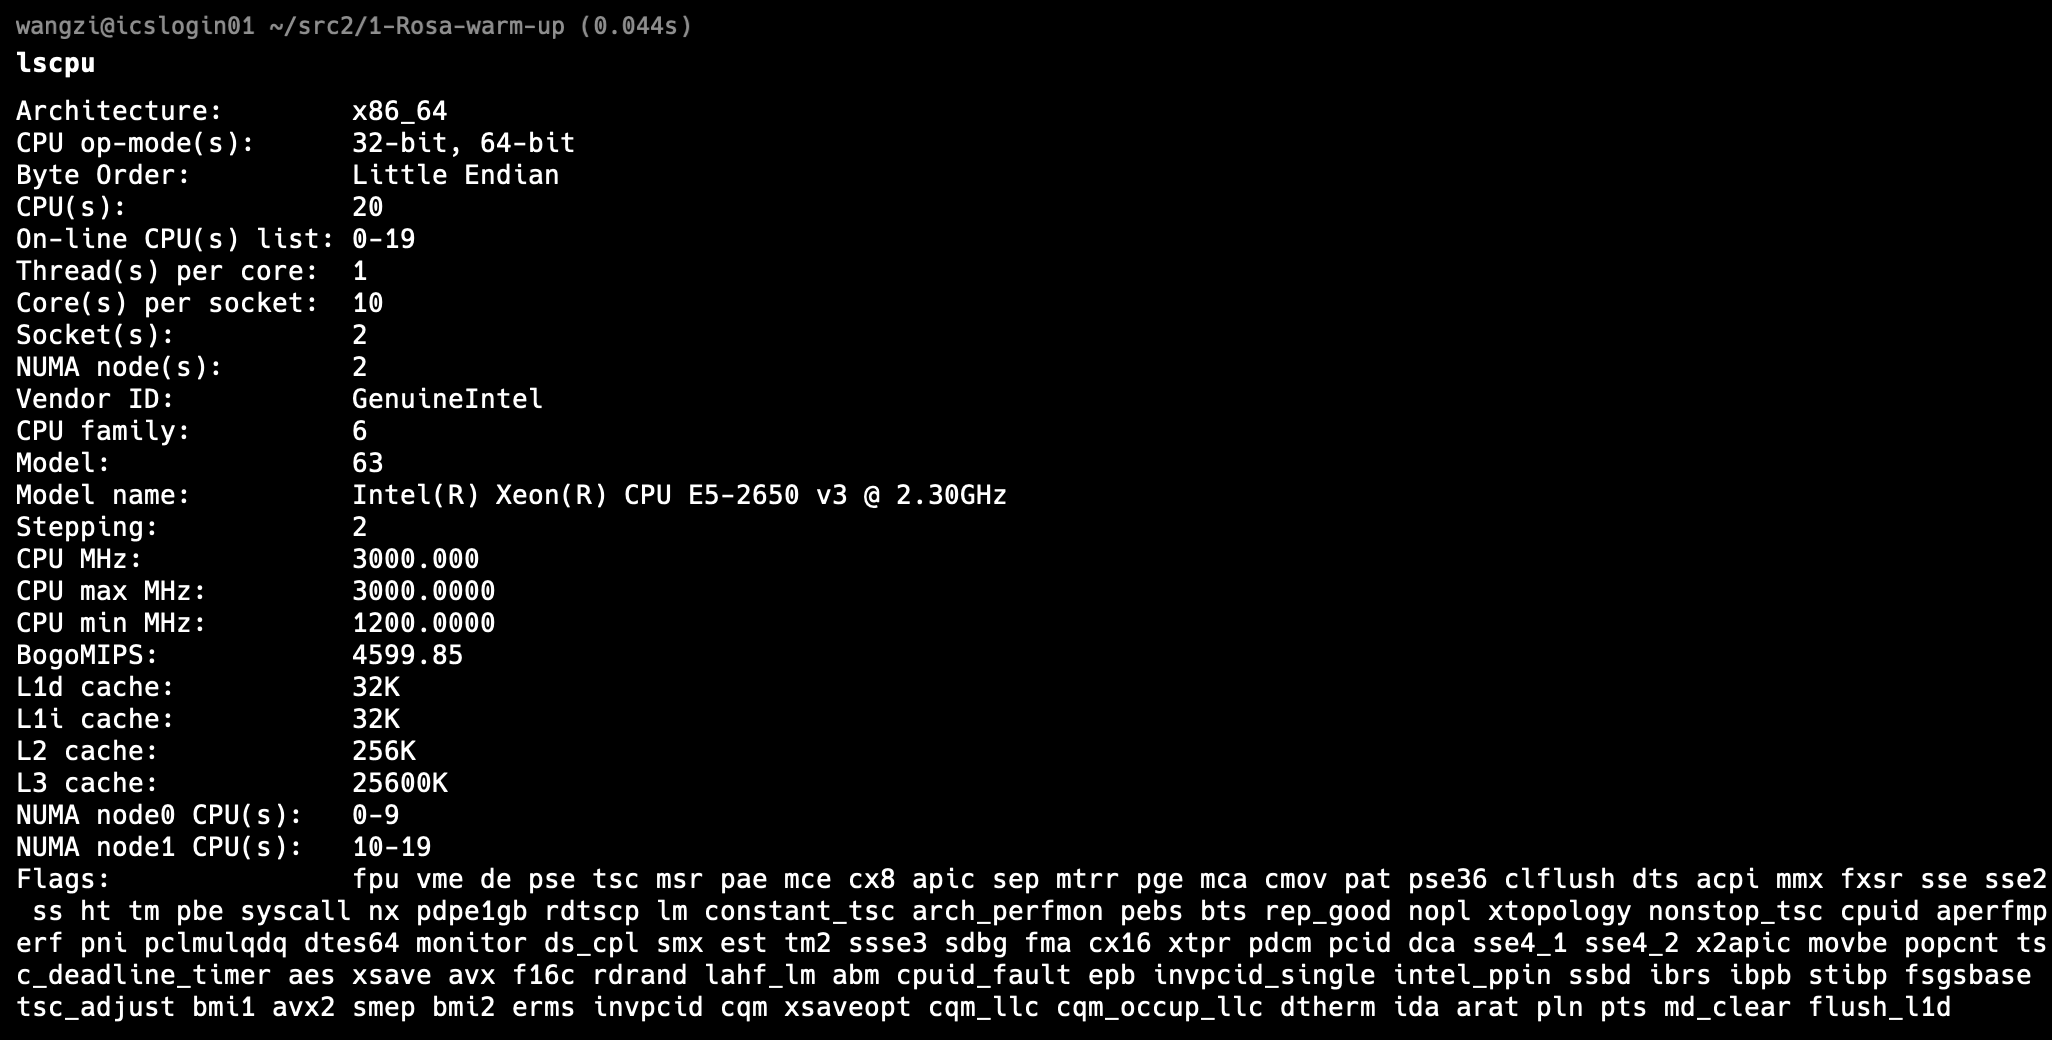
\includegraphics[width=0.8\textwidth]{pictures/lscpu.png}
%     \caption{Basic information of CPU}
% \end{figure}

To get the value of SIMD factor ($n_{\text{FMA}}$), we need to check on the \href{https://cpu-world.com}{cpu-world.com} website. The CPU of Rosa cluster is an Intel Xeon E5-2650, which has a core microarchitecture named Haswell. 
\begin{longtable}{|>{\raggedright\arraybackslash}p{4cm}|>{\raggedright\arraybackslash}p{2cm}|>{\raggedright\arraybackslash}p{2cm}|>{\raggedright\arraybackslash}p{2cm}|>{\raggedright\arraybackslash}p{4cm}|}
\hline
\textbf{Instruction} & \textbf{Lat} & \textbf{TP} & \textbf{Uops} & \textbf{Ports} \\
\hline
VFMADD132PD (XMM, XMM, M128) & [5;\(\leq\)11] & 0.50 / 0.50 & 1 / 2 & 1*p01+1*p23 \\
\hline
VFMADD132PD (XMM, XMM, XMM) & 5 & 0.50 / 0.50 & 1 / 1 & 1*p01 \\
\hline
VFMADD132PD (YMM, YMM, M256) & [5;\(\leq\)12] & 0.50 / 0.50 & 1 / 2 & 1*p01+1*p23 \\
\hline
\multicolumn{5}{|c|}{\dots} \\
\hline
\end{longtable}
The necessary data is available on the website, but it is too extensive to present in its entirety. The key point is that the TP values associated with the FMA operations remain consistent. As the Throughput (TP) is 0.50/0.50, then $n_{\text{FMA}} = \frac{1}{\text{TP}} = 2$.
% \begin{figure}[h]
%     \centering
%     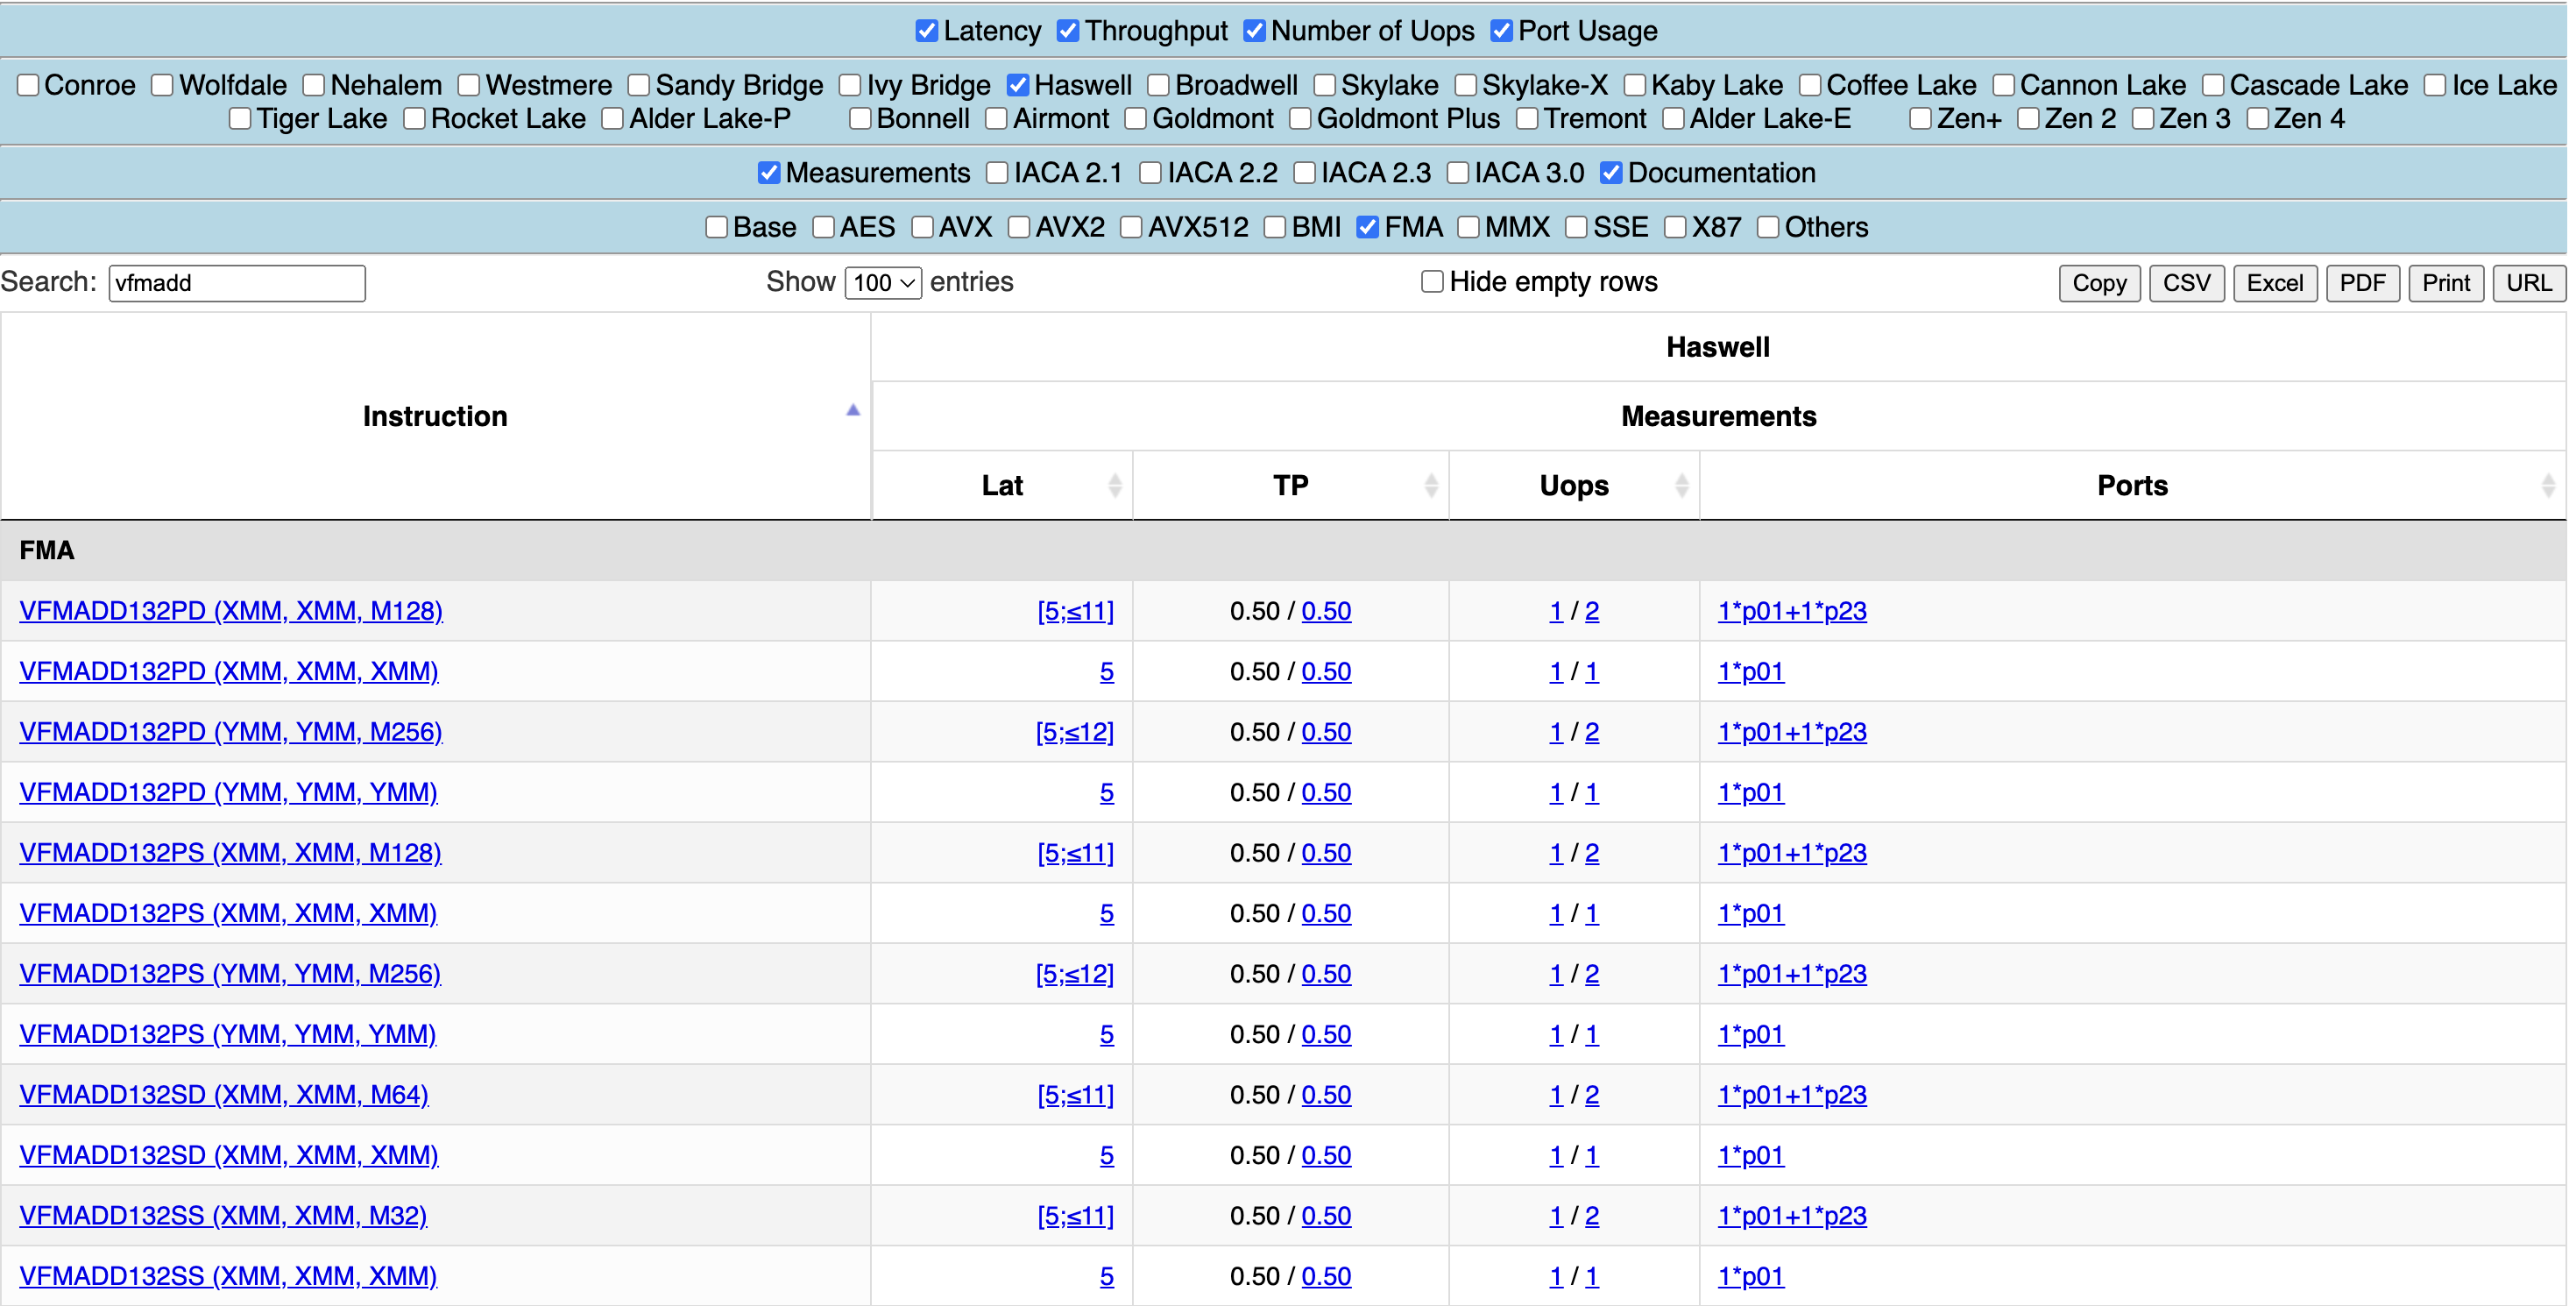
\includegraphics[width=0.8\textwidth]{pictures/uopsPart.png}
%     \caption{Part of uops table}
% \end{figure}

Based on above information, the value of Peak FLOPS as following:
\begin{equation}
    P_{\text{core}} = 2 \times 2 \times 4 \times 3.0\, \text{GHz} = 48\, \text{GFLOPS}
\end{equation}

\subsection{Cache and main memory size}
With batch \texttt{hwloc-ls}, we can see the structure of memory. The conclusions drawn are consistent with the teaching materials provided. In the structure diagram, L1 is divided into two parts, L1d (for data) and L1i (for instructions)\cite{L1}. In this work, only L1d needs to be considered.
\begin{figure}[h]
    \centering
    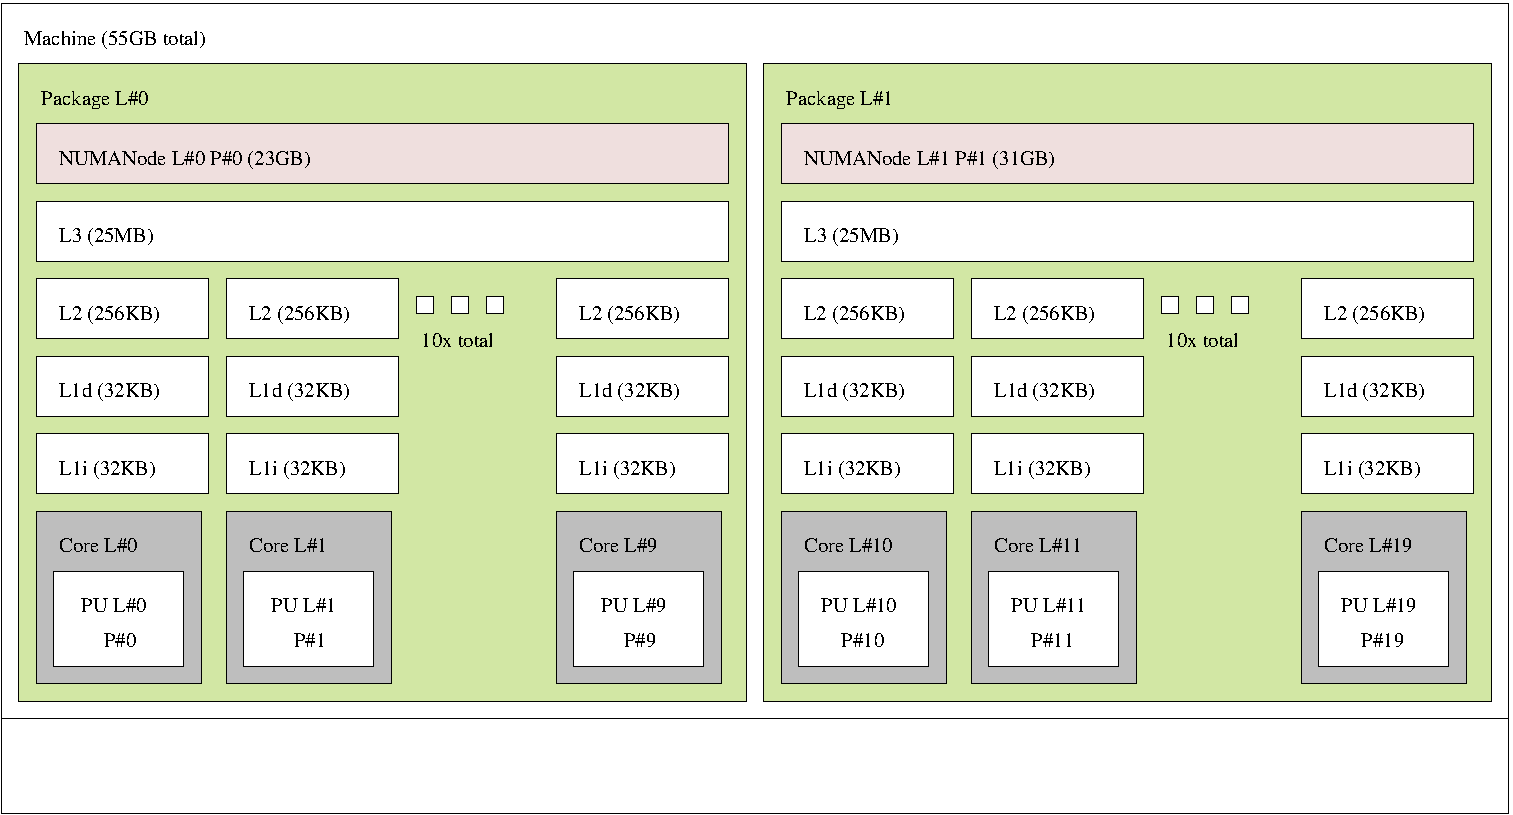
\includegraphics[width=0.8\textwidth]{pictures/XEON_E5-2650.pdf}
    \caption{Memory structure}
\end{figure}

\begin{table}[h]
    \centering
    \begin{tabular}{|c|c|}
        \hline
        \textbf{Component} & \textbf{Size} \\ 
        \hline
        Main memory & 23 GB \\ 
        \hline
        L3 cache & 25 MB \\ 
        \hline
        L2 cache & 256 KB \\ 
        \hline
        L1d cache & 32 KB \\ 
        \hline
    \end{tabular}
    \caption{Memory and Cache Sizes} 
    \label{tab:memory_cache} 
\end{table}


\subsection{Bandwidth}
First, we need confirm the value of $DSTREAM\_ARRAY\_SIZE$ is correct. Each array must be at least four times the size of the last cache level. 
\begin{equation}
    DSTREAM\_ARRAY\_SIZE \geq 4 \times \text{L3 Cache} = 4 \times 25 \, \text{MB} = 100 \, \text{MB}
\end{equation}
So $DSTREAM\_ARRAY\_SIZE$ needs to exceed 104,857,600 B. It is reasonable to set
\texttt{-DSTREAM\_ARRAY\_SIZE = 128000000} in the makefile.
\begin{lstlisting}[language=MyBatch, style=mystyle, caption={The makefile}]
CC = gcc
CFLAGS = -O3 -march=native -DSTREAM_TYPE=double -DNTIMES=20 

all: stream_c_1

stream_c_1: stream.c
    ${CC} ${CFLAGS} -DSTREAM_ARRAY_SIZE=128000000 stream.c -o stream_c_1

.PHONY: clean
clean:
    rm -f stream_c_1
# code from course material
\end{lstlisting}

The result after running is shown in the following table. As expected from the textbook, only the bandwidth of the copy operation shows a significant difference. It might because Copy kernel operations generally benefit from better cache utilization because of their simpler data access patterns. The data being copied may fit into the cache more effectively, minimizing cache misses and allowing faster memory access\cite{hager2010introduction}.

\begin{tabular}{|l|c|c|c|c|}
\hline
\textbf{Function} & \textbf{Best Rate MB/s} & \textbf{Avg time (s)} & \textbf{Min time (s)} & \textbf{Max time (s)} \\
\hline
Copy  & 19135.9 & 0.107083 & 0.107024 & 0.107272 \\
\hline
Scale & 11244.1 & 0.182227 & 0.182140 & 0.182403 \\
\hline
Add   & 12286.6 & 0.250114 & 0.250029 & 0.250248 \\
\hline
Triad & 12287.9 & 0.250091 & 0.250003 & 0.250243 \\
\hline
\end{tabular}
% \begin{figure}
%     \centering
%     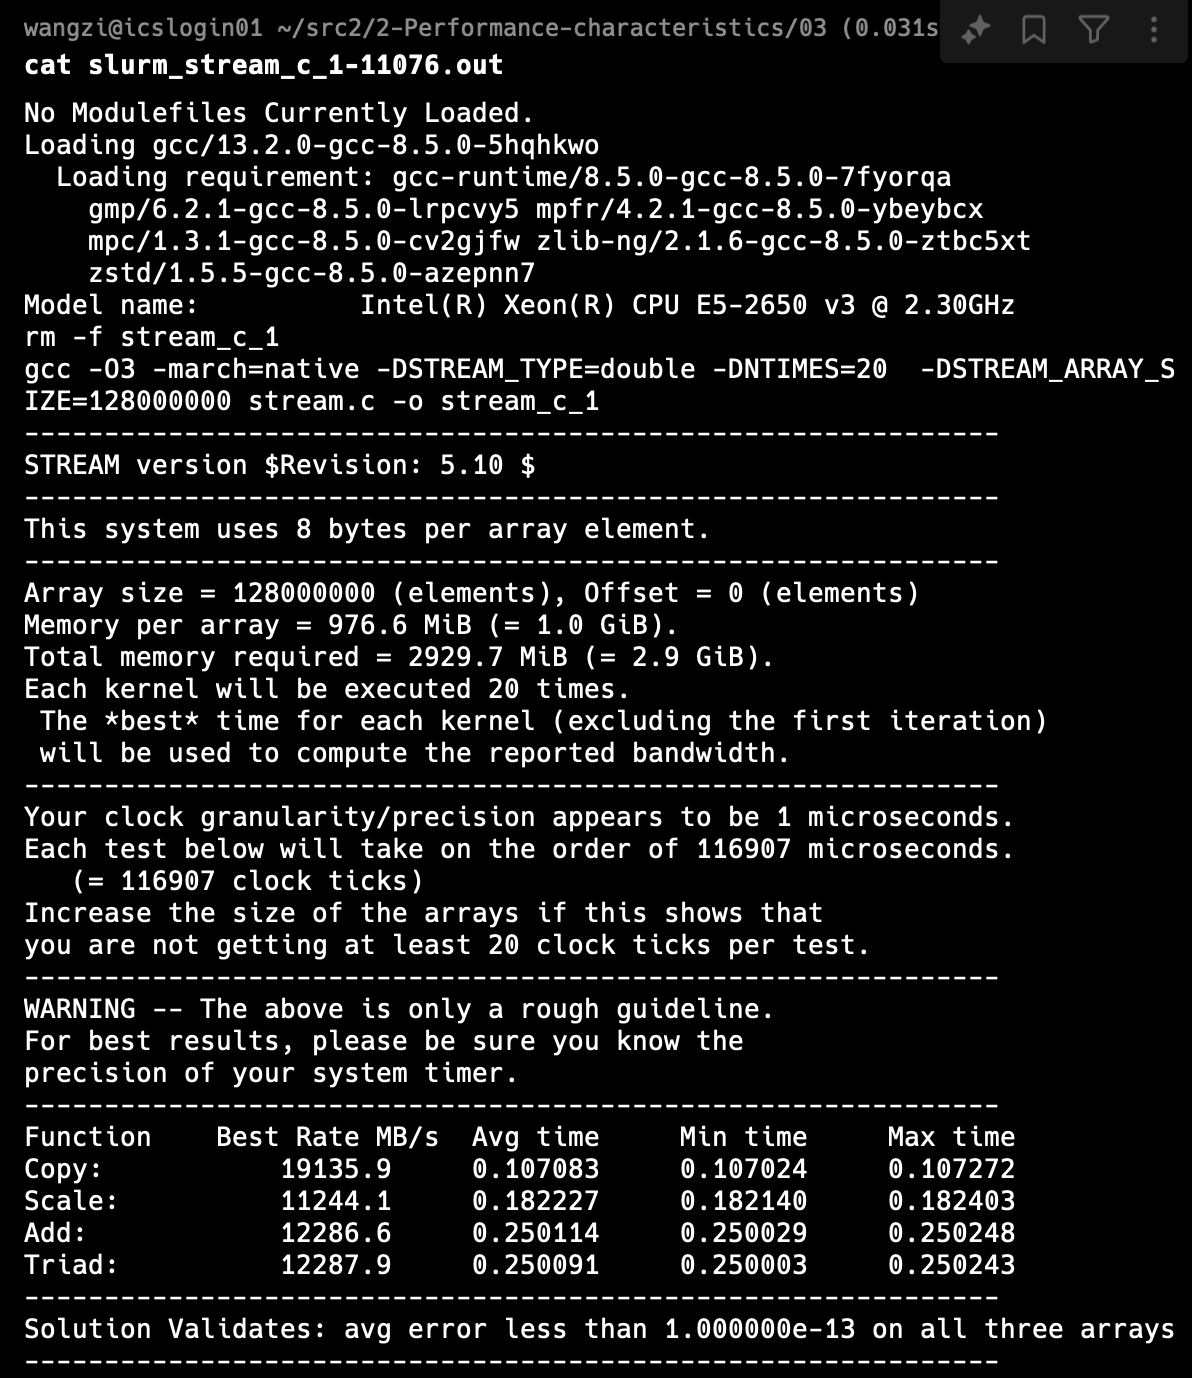
\includegraphics[width=0.8\textwidth]{pictures/Slurm output of STREAM benchmark.png}
%     \caption{Slurm output of STREAM benchmark}
% \end{figure}

As shown in the above table, the single-core bandwidth is approximately 12GB/s.


\subsection{Roofline model}
The important parameters required to build the model are as table 4. Replace the parameters in the example python file with it to get the desired Roofline model diagram. Two of the parameters, \( I_{\text{max}} \) and \( I_{\text{min}} \), are obtained from experience\cite{hager2010introduction}.

\begin{table}[h]
\centering
\begin{tabular}{|c|c|}
    \hline
    \textbf{Parameter} & \textbf{Value} \\
    \hline
    P\textsubscript{max} & 48 GFLOPS \\
    \hline
    b\textsubscript{max} & 12 GB/s \\
    \hline
    I\textsubscript{min} & 1.e-2 FLOPS/B \\
    \hline
    I\textsubscript{max} & 1.e+3 FLOPS/B \\
    \hline
\end{tabular}
\caption{Model parameters} 
\label{tab:memory_cache} 
\end{table}


\begin{figure}[h]
    \centering
    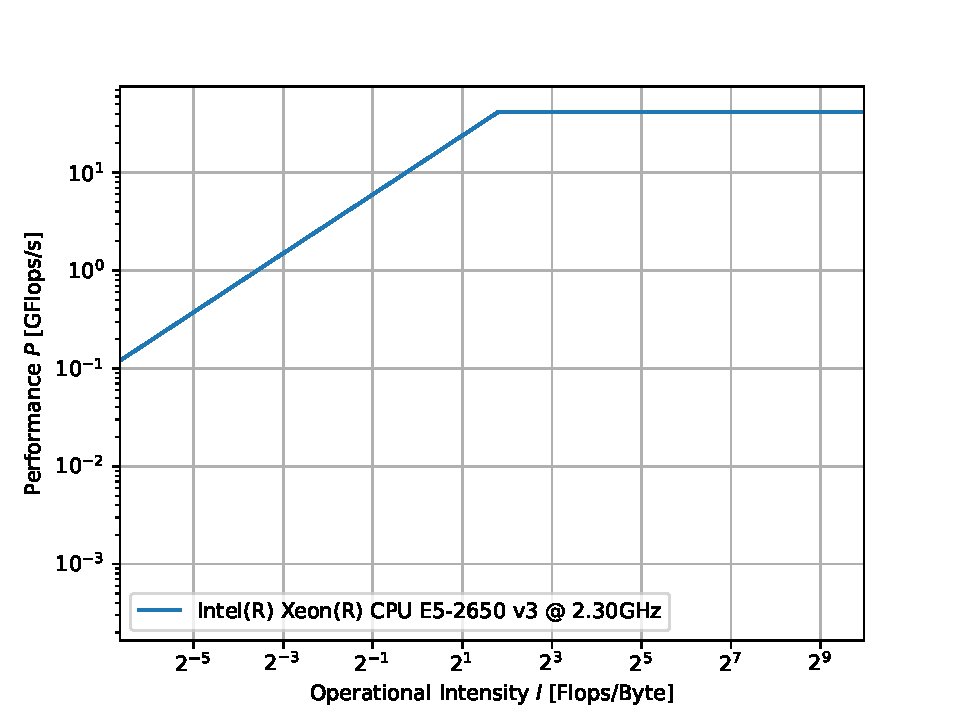
\includegraphics[width=0.8\textwidth]{pictures/roofline.pdf}
    \caption{Picture roofline model}
\end{figure}
In the picture 2, there is an obvious inflection point in the function. Using Formula 4, we can get the operating intensity inflection point value based on system performance.
\begin{equation}
    I_{\text{max}} = b_{\text{max}} \cdot P_{\text{max}} = \frac{42 \, \text{GFlops/s}}{12 \, \text{GB/s}} = 3.5 \, \text{FLOPS/Byte}
\end{equation}
\begin{itemize}
\item \textbf{Operation Intensity between 0.01 and 3.5 Flops/Byte}:
As operation intensity increases, performance improves but is still limited by memory bandwidth.
\item \textbf{Operation Intensity greater than 3.5 Flops/Byte}:
When operation intensity approaches 12 Flops/Byte, the system may become compute-bound.
\end{itemize}
\section{Optimize Square Matrix-Matrix Multiplication  \punkte{50}}
\subsection{Compiler options}
In this section, I will compare the running time of the program compiled with \texttt{-O0}, \texttt{-O2}, and \texttt{-O3} to evaluate the effect of compiler optimization. Initially, revising the makefile to compile the updated executable file.
\begin{lstlisting}[language=MyBatch, style=mystyle, caption={Makefile of Compiler options}]
OPT_O0 = -O0 -march=native       # No optimization, useful as a baseline
OPT_O1 = -O1 -march=native       # Moderate optimization level 1
OPT_O2 = -O2 -march=native       # Higher optimization level 2
CFLAGS_O0 = -Wall -std=gnu99 $(OPT_O0) # standard compiler flags with no optimization
CFLAGS_O1 = -Wall -std=gnu99 $(OPT_O1) # standard compiler flags with level 1 optimization
CFLAGS_O2 = -Wall -std=gnu99 $(OPT_O2) # standard compiler flags with level 2 optimization
\end{lstlisting}
Next step is to record new data time.
\begin{lstlisting}[language=MyBatch, style=mystyle, caption={Script of Compiler options}]
echo "==== benchmark-naive -O0 ===================="
srun ./benchmark-naive-O0 | tee timing_O0.data
echo

echo "==== benchmark-naive -O1 ===================="
srun ./benchmark-naive-O1 | tee timing_O1.data
echo

echo "==== benchmark-naive -O2 ===================="
srun ./benchmark-naive-O2 | tee timing_O2.data
echo

echo "==== benchmark-naive -O3 ===================="
srun ./benchmark-naive-O3 | tee timing_O3.data
echo
\end{lstlisting}
Finally, update recorded data to draw the picture.
\begin{lstlisting}[language=MyBatch, style=mystyle, caption={Plot of Compiler options}]
"timing_O0.data" using 2:4 title "Naive dgemm -O0" with linespoints pointtype 4 pointsize 2 linewidth 3 linetype 4 linecolor rgb "magenta", \
"timing_O1.data" using 2:4 title "Naive dgemm -O1" with linespoints pointtype 6 pointsize 2 linewidth 3 linetype 5 linecolor rgb "cyan", \
"timing_O2.data" using 2:4 title "Naive dgemm -O2" with linespoints pointtype 8 pointsize 2 linewidth 3 linetype 6 linecolor rgb "orange", \
"timing_O3.data" using 2:4 title "Naive dgemm -O3" with linespoints pointtype 3 pointsize 2 linewidth 3 linetype 7 linecolor rgb "black"
\end{lstlisting}
Due to the minimal impact of the compilation options on the final results, numerous data points overlap in the generated figure. Therefore, it is necessary to adjust the scale of the vertical axis. Then get the final result.
\begin{figure}
    \centering
    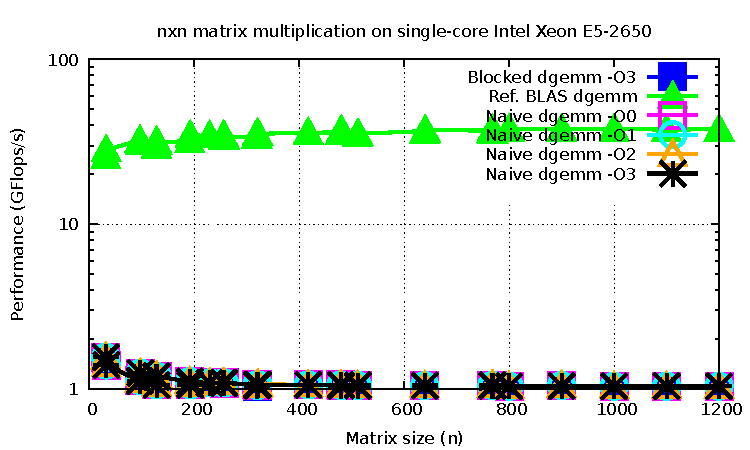
\includegraphics[width=0.8\textwidth]{pictures/timimg_Compile_options.pdf}
    
\end{figure}

\subsection{Tuning data access patterns}
In this section, I compare four approaches: the original OpenBLAS implementation (benchmark-blas) as a control group, an unoptimized naive implementation (benchmark-naive) for baseline comparison, an optimized naive implementation (benchmark-naive-tune) with data access pattern optimizations, and a blocked matrix multiplication implementation (benchmark-blocked) using block-level optimization techniques. As the procedure is similar to the previous case, detailed explanations will not be provided here.
\begin{figure}[h]
    \centering
    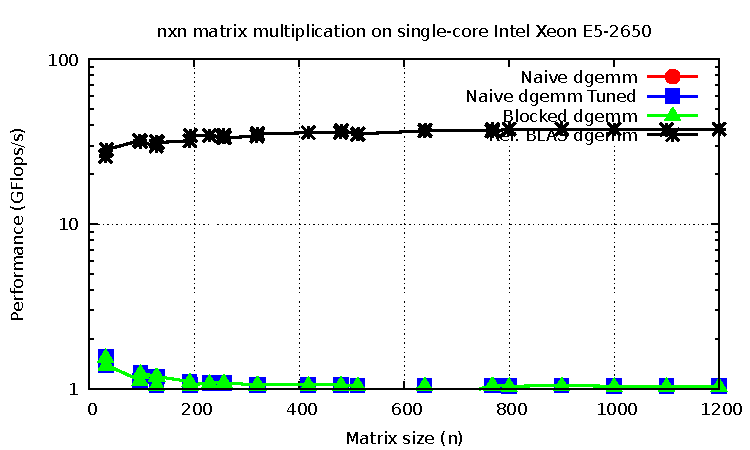
\includegraphics[width=0.8\textwidth]{pictures/timimg_data_access.pdf}
   
\end{figure}
\subsection{Vectorization}
In this section, I compare four methods: Naive dgemm Vectorized, a vectorized version of the naive implementation; Blocked dgemm Vectorized, a vectorized version of the blocked matrix multiplication; OpenBLAS Vectorized, a vectorized implementation of OpenBLAS; and Ref. BLAS dgemm (original), the unmodified OpenBLAS implementation used as a control group. As the procedure is similar to the previous case, detailed explanations will not be provided here.
\begin{figure}[h]
    \centering
    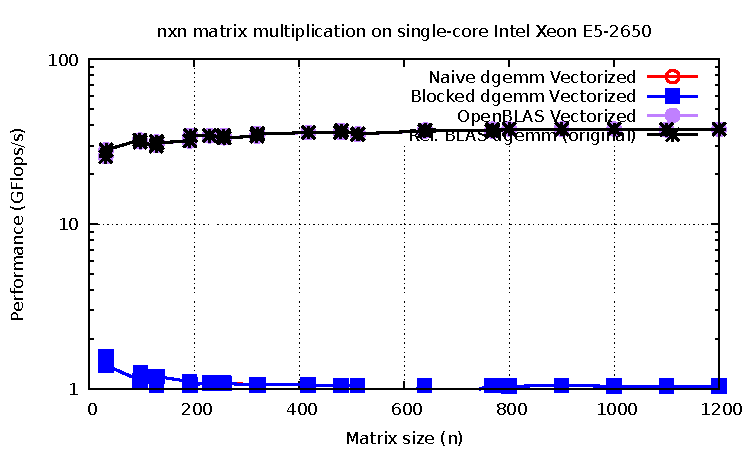
\includegraphics[width=0.8\textwidth]{pictures/timimg_Vectorization.pdf}
    
\end{figure}
\subsection{Loop unrolling}
This section compares four methods: benchmark-naive-unrolled, a naive implementation with loop unrolling; benchmark-blocked-unrolled, a blocked matrix multiplication with loop unrolling; benchmark-blas-unrolled, an OpenBLAS implementation with loop unrolling; and benchmark-blas, the original OpenBLAS implementation used as a control group. As the procedure is similar to the previous case, detailed explanations will not be provided here.
\begin{figure}[h]
    \centering
    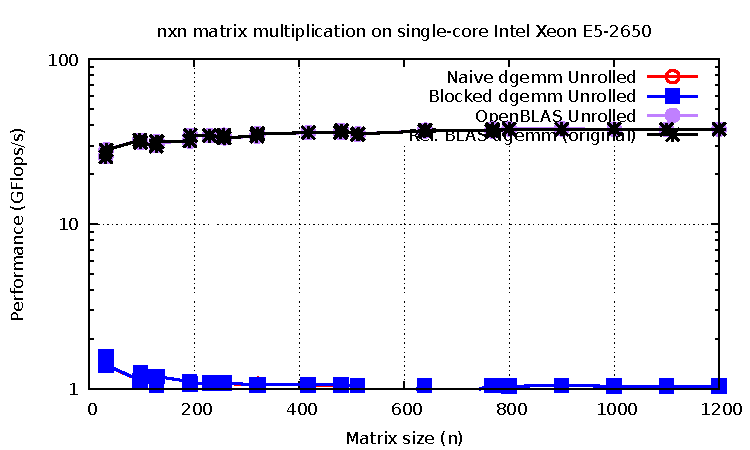
\includegraphics[width=0.8\textwidth]{pictures/timimg_loop copy.pdf}
    
\end{figure}
\printbibliography
\appendix
\section{Appendix: Code}
\begin{lstlisting}[language=MyC++, style=mystyle, caption={Hello World Program}]
#include <cstdlib>
#include <iostream>
    
using namespace std;
    
int main() {
    const char *nodes = std::getenv("SLURM_JOB_NODELIST");
    cout << "Hello World" << '\n';
    cout << "host(node) name:" << nodes << '\n';
    return 0;
}
//for each print, read the host name
\end{lstlisting}

\begin{lstlisting}[language=MyBatch, style=mystyle, caption={Tmakefile of Compiler options}]
#!/bin/bash
#SBATCH --job-name=slurm_job_one      # Job name    (default: sbatch)
#SBATCH --output=slurm_job_one-%j.out # Output file (default: slurm-%j.out)
#SBATCH --error=slurm_job_one-%j.err  # Error file  (default: slurm-%j.out)
#SBATCH --ntasks=1                    # Number of tasks
#SBATCH --cpus-per-task=1             # Number of CPUs per task
#SBATCH --time=00:01:00               # Wall clock time limit
#SBATCH --partition=slim                 
#SBATCH --nodelist=icsnode25             

# load some modules & list loaded modules
module load gcc
module list

# print CPU model
lscpu | grep "Model name"

# run (srun: run job on cluster with provided resources/allocation)
srun ./hello_worldc

\end{lstlisting}

\begin{lstlisting}[language=MyBatch, style=mystyle, caption={The batch script of two node}]
#!/bin/bash
#SBATCH --job-name=slurm_job_two      # Job name    (default: sbatch)
#SBATCH --output=slurm_job_two-%j.out # Output file (default: slurm-%j.out)
#SBATCH --error=slurm_job_two-%j.err  # Error file  (default: slurm-%j.out)
#SBATCH --nodes=2                     # Number of nodes
#SBATCH --ntasks=2                    # Number of tasks
#SBATCH --cpus-per-task=1             # Number of CPUs per task
#SBATCH --time=00:01:00               # Wall clock time limit
#SBATCH --partition=slim 
#SBATCH --nodelist=icsnode26,icsnode27

# load some modules & list loaded modules
module load gcc
module list

# print CPU model
lscpu | grep "Model name"

# run (srun: run job on cluster with provided resources/allocation)

\end{lstlisting}

\begin{lstlisting}[language=MyBatch, style=mystyle, caption={The batch scripts of STREAM benchmark}]
#!/bin/bash
#SBATCH -A es_math                       # Account (es_math or ls_math)
#SBATCH --job-name=slurm_stream_c_1      # Job name    (default: sbatch)
#SBATCH --output=slurm_stream_c_1-%j.out # Output file (default: slurm-%j.out)
#SBATCH --error=slurm_stream_c_1-%j.err  # Error file  (default: slurm-%j.out)
#SBATCH --ntasks=1                       # Number of tasks
#SBATCH --cpus-per-task=1                # Number of CPUs per task
#SBATCH --time=00:01:00                  # Wall clock time limit

# load some modules & list loaded modules
module list
module load gcc

# print CPU info
lscpu | grep "Model name"

# compile & run
make clean
make
srun ./stream_c_1
# code from course material
\end{lstlisting}

\begin{lstlisting}[language=MyPython, style=mystyle, caption={Draw the picture roofline model}]
import matplotlib.pyplot as plt
import numpy as np


def plot_roofline(Pmax, bmax, Imin, Imax, N=1000, ax=None, **plt_kwargs):
    if ax is None:
        ax = plt.gca()
    I = np.logspace(np.log(Imin), np.log(Imax), N)
    P = bmax * I
    P = np.minimum(P, Pmax)
    ax.loglog(I, P, **plt_kwargs)
    ax.set_xscale('log', base=2)
    # ax.set_yscale('log', base=2)
    ax.grid(True)
    ax.set_xlim(Imin, Imax)
    ax.set_xlabel(rf"Operational Intensity $I$ [Flops/Byte]")
    ax.set_ylabel(rf"Performance $P$ [GFlops/s]")
    return ax


if __name__ == "__main__":
    fig, ax = plt.subplots()
    ax = plot_roofline(Pmax=42, bmax=12, Imin=1.e-2, Imax=1.e+3, ax=ax,
                        label="Intel(R) Xeon(R) CPU E5-2650 v3 @ 2.30GHz")
    ax.legend()
    plt.savefig("roofline.pdf")
    plt.show()
* code from course material
\end{lstlisting}


\section{Appendix: Terminal Output}
\begin{lstlisting}[style=mystyle, language=MyBash,caption={Basic information of nodes}]
wangzi@icslogin01 ~ (0.055s)
sinfo
PARTITION  AVAIL   TIMELIMIT     NODES    STATE NODELIST
slim*      up      2-00:00:00    8        plnd icsnodel [19-261]
slim*      up      2-00:00:00    7        mix icsnode[17-18, 32-361]
slim*      up      2-00:00:00    2        alloc icsnode[37-381]
gpu        up      2-00:00:00    1        idle icsnode[27-31]
gpu        up      2-00:00:00    1        mix icsnode05
gpu        up      2-00:00:00    8        alloc icsnode06
gpu        up      2-00:00:00    4        idle icsnodel [08-15]
bigMem     up      2-00:00:00    2        idle icsnode[01-04]
bigMem     up      2-00:00:00    2        idle icsnode[07, 15]
debug-slim up      4:00:00       1        idle icsnode39
debug-gpu  up      4:00:00       1        plnd icsnode16
multi_gpu  up      2-00:00:00    2        idle icsnode[41-42]
\end{lstlisting}

\begin{lstlisting}[language=MyBatch, style=mystyle, caption={The Result of batch script of one node}]
wangzi@icslogin01 ~/src2/1-Rosa-warm-up (0.0295)
cat slurm_job_one-10854.out
Currently Loaded Modulefiles:
1) gec-runtime/8.5.0-gcc-8.5.0-7fyorqa
2) gmp/6.2.1-gcc-8.5.0-1rpcvy5
3) mpfr/4.2.1-gcc-8.5.0-ybeybcx
4) mpc/1.3.1-gcc-8.5.0-cv2gjfw
5) zlib-ng/2.1.6-gcc-8.5.0-ztbc5xt
6) zstd/1.5.5-gcc-8.5.0-azepnn7
7) gcc/13.2.0-gcc-8.5.0-5hqhkwo
Model name:
Intel(R) Xeon(R) CPU E5-2650 v3 @ 2.30GHz
Hello World
host(node) name: icsnode25
\end{lstlisting}

\begin{lstlisting}[style=mystyle, caption={The Result of batch script of two node}]
wangzi@icslogin01 ~/src2/1-Rosa-warm-up (0.0295)
cat slurm_job_two-10873.out
Currently Loaded Modulefiles:
1) gec-runtime/8.5.0-gcc-8.5.0-7fyorqa
2) gmp/6.2.1-gcc-8.5.0-1rpcvy5
3) mpfr/4.2.1-gcc-8.5.0-ybeybcx
4) mpc/1.3.1-gcc-8.5.0-cv2gjfw
5) zlib-ng/2.1.6-gcc-8.5.0-ztbc5xt
6) zstd/1.5.5-gcc-8.5.0-azepnn7
7) gcc/13.2.0-gcc-8.5.0-5hqhkwo
Model name:
Intel(R) Xeon(R) CPU E5-2650 v3 @ 2.30GHz
Hello World
host(node) name: icsnode[26-27]
Hello World
host(node) name: icsnode[26-27]
\end{lstlisting}

\end{document}